% Chapter nc_iw: Iwaniec's approach and the level of the Thorin measure (Volume II, after the quasi Riemann hypothesis chapter nc_qrh).
% Based on an unrefereed note of N. G. Polson (November 2026), rewritten in the book's form with the corrections of the referee reports misc/research/directions/opus/IW1.md and IW2.md.
% Numbers: the computed values are those of the note, rechecked independently by the referee for zeta, L(s,chi_{-4}), five of the twelve curves and the level explicit formula (see the reports); status words as in the rest of the book.

This chapter places the approach to the Landau Siegel zero and to a quasi Riemann hypothesis that Iwaniec described, as reported by Conrey, inside the Thorin framework of the two volumes. It is based on an unrefereed note of Polson (November 2026), reworked here in the book's form and corrected after a referee's reading. Its central statement is a dictionary (Theorem~\ref{iw:thm:dictionary}): for an admissible $L$ function $\Lambda$ and a level $\alpha\ge\frac12$, the function $\Lambda(\alpha)/\Lambda(\alpha+\sqrt s)$ is the Laplace transform of a generalised gamma convolution if and only if $\Lambda$ has no zero with real part above $\alpha$. For $\xi$ this is Theorem~\ref{thm:poisson}, which we cite and do not reprove; what is added is the extension to Dirichlet $L$ functions and elliptic curve $L$ functions, with the factor lemma that gives the explicit density. Around it: the Cauchy semigroup (cited from Theorem~\ref{tf:thm:poisson}), the growth of the Thorin mass, a level $\alpha$ explicit formula with a residue identity and a level average that contains Weil's functional, three readings of arithmetic quantities at the origin of the measure (rank, a Landau Siegel zero, central values), computed tables, and a short honest answer to the question whether any of this is a path to the Riemann hypothesis. It is not.

Every result carries one of the status words proved, computed, conditional, heuristic or open. The unrefereed zero free half plane $\re s>\frac78$ of \cite{OAI26a} is never used as a theorem; statements that use it are conditional and say so. No priority is claimed for anything below.

\section{Iwaniec's approach, as reported}\label{iw:sec:approach}

% UNCHECKED: Conrey survey text not read
Iwaniec lectured on his approach at the third conference on the Riemann hypothesis, and Conrey's survey \cite{NCConrey03} describes the lecture. We have not read the survey, and what follows is the account of the source note, offered as reported by Conrey, with the status heuristic. Take a family of $L$ functions with a multiple zero at $s=\frac12$ and approximate the M\"obius function $\mu(n)$ by linear combinations of the coefficients of the family, which tames $\mu$. The model family is the set of elliptic curves
\[
E_{A,B^2}:\ y^2=x^3+Ax+B^2 .
\]
The point $(0,B)$ lies on each curve. When it has infinite order the rank is at least one, the analytic rank is then at least one (Gross, Zagier and Kolyvagin \cite{NCGrossZagier86,NCKolyvagin89}, for modular curves), and for $A,B$ in suitable progressions the root number is $+1$, which forces a central zero of order at least two. Iwaniec formulated three conjectures which together would exclude a Landau Siegel zero, and harder constructions of the same kind would give a quasi Riemann hypothesis, a concrete $\beta<1$ with no zero to the right of $\re s=\beta$. Iwaniec's own account is \cite{NCIwaniecConv06}, which we have not read (we do not know whether it describes this family), and a related route through small gaps between zeros is in \cite{NCConreyIwaniec02}.

A caution. If $(0,B)$ has infinite order, then $L(E,1)=0$ for every curve of the family, whatever the root number, so the central value in the setting below is zero throughout. The moment that Iwaniec bounds must therefore be one of a derivative or of a different family; the source note's formula for it could not be confirmed and is not reproduced. The aim here is only to say precisely what Iwaniec's target means for the Thorin programme: the statement that $\varphi_\alpha$ is a GGC transform at a level $\alpha$ below one.

\section{Setting and the factor lemma}\label{iw:sec:setting}

\begin{definition}
An \emph{admissible $L$ function} is one of the following completed functions: $\xi(s)=\frac12s(s-1)\pi^{-s/2}\Gamma(s/2)\zeta(s)$; $\Lambda(s,\chi)=(q/\pi)^{(s+\mathfrak a)/2}\Gamma\big(\frac{s+\mathfrak a}{2}\big)L(s,\chi)$ for a real primitive character $\chi$ modulo $q>1$ with $\chi(-1)=(-1)^{\mathfrak a}$; or, for an elliptic curve $E/\mathbb Q$ of conductor $N$, $\Lambda_E(s)=N^{s/2}(2\pi)^{-s-1/2}\Gamma(s+\frac12)L(E,s+\frac12)$, in the normalisation with centre $\frac12$. For a complex character one uses the product $\Lambda(s,\chi)\Lambda(s,\bar\chi)$.
\end{definition}

An admissible $\Lambda$ is entire of order one and real on $\R$, satisfies $\Lambda(1-s)=\pm\Lambda(s)$, and has its zeros $\rho=\beta+i\gamma$ in the strip $0<\beta<1$ (for $\Lambda_E$ this uses the nonvanishing of the $L$ function on the edge of the strip). The zero set is invariant under $\rho\mapsto\bar\rho$ and $\rho\mapsto1-\rho$. By the Hadamard product \cite[Ch.~12]{Davenport}, \cite[Thm.~5.6]{IwaniecKowalski04}, and since $\Lambda$ is real on $\R$, summing over conjugate pairs gives
\begin{align}
\frac{\Lambda'}{\Lambda}(s)&=\sum_\rho\frac1{s-\rho}\qquad(\text{conjugate pairs together}),\label{iw:eq:logderiv}\\
\re\frac{\Lambda'}{\Lambda}(\sigma+it)&=\sum_\rho\frac{\sigma-\beta}{(\sigma-\beta)^2+(t-\gamma)^2}\qquad(\text{absolutely convergent}).\label{iw:eq:relogderiv}
\end{align}
For $\alpha\ge\frac12$ with $\Lambda(\alpha)\ne0$ the \emph{level $\alpha$ Thorin function} is $\varphi_\alpha(s)=\Lambda(\alpha)/\Lambda(\alpha+\sqrt s)$ on $\mathbb C\setminus(-\infty,0]$, with the principal root, and $\mathrm{QRH}(\alpha)$ is the statement that $\Lambda$ has no zero with $\re\rho>\alpha$. A probability law on $[0,\infty)$ is a generalised gamma convolution (GGC) when its Laplace transform is $\exp\{-as-\int_{(0,\infty)}\log(1+s/t)\,U(dt)\}$ with $a\ge0$ and a nonnegative Thorin measure $U$ with $\int_{(0,1]}|\log t|\,U(dt)+\int_{(1,\infty)}t^{-1}U(dt)<\infty$. We use three standard facts \cite{Bondesson}: the transform extends analytically and without zeros to $\mathbb C\setminus(-\infty,0]$; the class is closed under products, with Thorin measures adding; and it is closed under weak limits, with Thorin measures converging vaguely.

\begin{lemma}[factor lemma]\label{iw:lem:factor}
Let $\gamma\ne0$ and $\delta$ be real and $f(s)=\dfrac{\delta^2+\gamma^2}{(\sqrt s+\delta)^2+\gamma^2}$.
\begin{enumerate}
\item[(i)] If $\delta\ge0$, $f$ is the Laplace transform of a GGC with $a=0$ and a Thorin measure of total mass one. For $\delta>0$ its density is
\begin{equation}\label{iw:eq:factordensity}
\begin{split}
u(t)&=\frac{\delta(\delta^2+\gamma^2+t)}{\pi\sqrt t\,\big[(\delta^2+\gamma^2-t)^2+4\delta^2t\big]}\\
&=\frac1{2\pi\sqrt t}\Big[\frac{\delta}{\delta^2+(\sqrt t-\gamma)^2}+\frac{\delta}{\delta^2+(\sqrt t+\gamma)^2}\Big],
\end{split}
\end{equation}
and for $\delta=0$ the Thorin measure is the unit atom at $\gamma^2$, the weak limit of \eqref{iw:eq:factordensity} as $\delta\downarrow0$.
\item[(ii)] If $\delta<0$, $f$ has poles at $s=(-\delta\pm i\gamma)^2\in\mathbb C\setminus(-\infty,0]$ and is not a GGC transform.
\item[(iii)] For $\delta>0$, $g(s)=\delta/(\delta+\sqrt s)$ is a GGC transform with $a=0$ and Thorin density $\delta/\big(2\pi\sqrt t(\delta^2+t)\big)$, of total mass $\frac12$. For $\delta<0$, $g$ has a pole at $s=\delta^2>0$ and is not a GGC transform.
\end{enumerate}
Status: proved.
\end{lemma}

\begin{proof}
(i) Put $w=\sqrt z$. The zeros of $(w+\delta)^2+\gamma^2$ are $w=-\delta\pm i\gamma$, with $\re w\le0$, so for $\delta>0$ the function $f$ is analytic and zero free on $\mathbb C\setminus(-\infty,0]$, and $S(z):=-f'(z)/f(z)=\dfrac{w+\delta}{w((w+\delta)^2+\gamma^2)}$ is analytic there, positive on $(0,\infty)$, $O(|z|^{-1})$ at infinity and $O(|z|^{-1/2})$ at the origin. Cauchy's formula on a keyhole contour round $(-\infty,0]$ gives $S(z)=\int_0^\infty u(t)(t+z)^{-1}dt$ with $u(t)=\pi^{-1}\Im S(-t-i0)$. On the lower edge $w=-iy$, $y=\sqrt t$, a direct computation gives $\Im S(-t-i0)=\delta(\delta^2+y^2+\gamma^2)/\big(y[(\delta^2+\gamma^2-y^2)^2+4\delta^2y^2]\big)$, the first form of \eqref{iw:eq:factordensity}; the second follows from $(\delta^2+(y-\gamma)^2)(\delta^2+(y+\gamma)^2)=(\delta^2+\gamma^2-y^2)^2+4\delta^2y^2$. Integrating $S$ along $[0,s]$ and using $f(0)=1$ gives $-\log f(s)=\int_0^\infty\log(1+s/t)u(t)\,dt$, so $a=0$, and the mass is $\lim_{z\to+\infty}zS(z)=1$. In the variable $y$ the measure is the sum of two Cauchy densities of width $\delta$ centred at $\pm\gamma$ restricted to $y>0$, which tends weakly to $\delta_\gamma$ as $\delta\downarrow0$; the case $\delta=0$ is the gamma transform $\gamma^2/(\gamma^2+s)$.

(ii) The zero $w=-\delta+i\gamma$ of the denominator has $\re w>0$ and is not purely imaginary, so $s=w^2\notin(-\infty,0]$ is a pole on the principal sheet. (iii) Here $S(z)=1/(2w(w+\delta))$, the same computation gives the density, and the mass is $\lim zS(z)=\frac12$. For $\delta<0$ the pole $\sqrt s=-\delta>0$ gives $s=\delta^2>0$.
\end{proof}

\section{The dictionary}\label{iw:sec:dictionary}

\begin{theorem}[level $\alpha$ dictionary]\label{iw:thm:dictionary}
Let $\Lambda$ be admissible and $\alpha\ge\frac12$ with $\Lambda(\alpha)\ne0$. The following are equivalent.
\begin{enumerate}
\item[(a)] $\mathrm{QRH}(\alpha)$.
\item[(b)] $\varphi_\alpha$ is the Laplace transform of a GGC.
\item[(c)] $\re(\Lambda'/\Lambda)(s)>0$ whenever $\re s>\alpha$.
\end{enumerate}
When they hold, $a=0$ and the Thorin measure $U_\alpha$ is the sum of the factor measures of Lemma~\ref{iw:lem:factor} with $\delta=\alpha-\beta$, one for each conjugate pair of zeros (mass one) and one for each real zero (mass $\frac12$). Off the atoms at $\gamma^2$ contributed by zeros on the line $\re s=\alpha$, it has density
\begin{equation}\label{iw:eq:thorindensity}
u_\alpha(t)=\frac1{2\pi\sqrt t}\,\re\frac{\Lambda'}{\Lambda}\big(\alpha+i\sqrt t\big).
\end{equation}
Status: proved.
\end{theorem}

For $\xi$ the equivalence of (a) and (b) is Theorem~\ref{thm:poisson}, with density \eqref{eq:rho} at $\varepsilon=\alpha-\frac12$.

\begin{proof}
By \eqref{iw:eq:logderiv}, $B_\alpha:=\Lambda'/\Lambda(\alpha)=\sum_\rho(\alpha-\rho)^{-1}$. Expanding the Hadamard product about $\alpha$ with $c_\rho=\rho-\alpha$, the exponential factors cancel when conjugate pairs are grouped, and
\[
\frac{\Lambda(\alpha+w)}{\Lambda(\alpha)}=\prod_{\gamma>0}\Big(1-\frac w{c_\rho}\Big)\Big(1-\frac w{\bar c_\rho}\Big)\prod_{\gamma=0}\Big(1-\frac w{c_\rho}\Big),
\]
absolutely convergent because $\sum_{\gamma>0}|\re c_\rho|/|c_\rho|^2<\infty$ and $\sum|c_\rho|^{-2}<\infty$. With $w=\sqrt s$, each pair factor is the reciprocal of the $f$ of Lemma~\ref{iw:lem:factor} with $\delta=\alpha-\beta$, and each real zero factor the reciprocal of its $g$, so $\varphi_\alpha=\prod_\rho f_\rho$.

(a)$\Rightarrow$(b). By the functional equation $1-\alpha\le\beta\le\alpha$, so every $\delta_\rho\ge0$, and real zeros have $\beta<\alpha$ because $\Lambda(\alpha)\ne0$. Each factor, hence each finite partial product, is a GGC transform. The partial products converge pointwise to $\varphi_\alpha$ and $\varphi_\alpha(s)\to1$ as $s\downarrow0$, so by the continuity theorem $\varphi_\alpha$ is the transform of a law, GGC by closure under weak limits, with $U_\alpha$ the sum of the factor measures by vague convergence. The drift vanishes since $\log\Lambda(\alpha+\sqrt s)=O(\sqrt s\log s)=o(s)$ for a function of order one.

(b)$\Rightarrow$(a). A zero with $\beta>\alpha$ gives $\varphi_\alpha$ a pole off $(-\infty,0]$ by Lemma~\ref{iw:lem:factor}(ii) and (iii) (a pair, or a real zero, with $\delta<0$), and a GGC transform has none there.

(a)$\Rightarrow$(c). In \eqref{iw:eq:relogderiv} with $\sigma>\alpha\ge\beta$ every term is positive.

(c)$\Rightarrow$(a). This is Lagarias's argument \cite{Lagarias} moved from $\frac12$ to $\alpha$. If $\rho_0$ has multiplicity $m$ and $\beta_0>\alpha$, then $\Lambda'/\Lambda(s)=m/(s-\rho_0)+O(1)$ near $\rho_0$, which tends to $-\infty$ along $s=\rho_0-\varepsilon$, $\varepsilon\downarrow0$, and these points have $\re s>\alpha$.

Finally, summing the second form of \eqref{iw:eq:factordensity} over all zeros and comparing with \eqref{iw:eq:relogderiv} at $\alpha+i\sqrt t$ gives \eqref{iw:eq:thorindensity}, the interchange being justified by absolute convergence.
\end{proof}

\begin{remark}[complex characters paired with their conjugates]\label{iw:rem:complexchar}
Let $\chi$ be a primitive nontrivial Dirichlet character that is not real, with completed function $\Lambda(s,\chi)$ entire of order one, let $\alpha\ge\frac12$ and $L(\alpha,\chi)\ne0$ (hence $L(\alpha,\bar\chi)\ne0$). Put $F_{\alpha,\chi}(s)=\Lambda(\alpha,\chi)\Lambda(\alpha,\bar\chi)/\big(\Lambda(\alpha+\sqrt s,\chi)\Lambda(\alpha+\sqrt s,\bar\chi)\big)$. Then $F_{\alpha,\chi}$ is the Laplace transform of a GGC if and only if $L(s,\chi)$ has no zero with $\re s>\alpha$. The zeros of $L(s,\bar\chi)$ are the conjugates $\bar\rho$ of those of $L(s,\chi)$, so $\rho$ and $\bar\rho$ together form the conjugate pair that Lemma~\ref{iw:lem:factor} requires, with $\delta=\alpha-\beta$ (for a real zero, part (iii) applied twice), and the proof of Theorem~\ref{iw:thm:dictionary} applies to the product: the exponential factors cancel in the Hadamard product because the constant in $\Lambda(s,\chi)=e^{A(\chi)+B(\chi)s}\prod_\rho(1-s/\rho)e^{s/\rho}$ satisfies $\re B(\chi)=-\sum_\rho\re\rho^{-1}$ for primitive $\chi$ \cite[Ch.~12]{Davenport} (this is where primitivity is used), the product converges absolutely since $\sum_\rho|\rho-\alpha|^{-2}<\infty$, and a pair with $\gamma\ge2$ contributes $\ll_\alpha\gamma^{-2}$ to $\int_{(1,\infty)}t^{-1}U(dt)$, since $0\le\alpha-\beta\le\alpha$, which is summable. The functional equation exchanges the zeros of $L(s,\chi)$ with the reflected conjugates $1-\bar\rho$ of its own zeros, so $1-\alpha\le\beta$ whenever there is no zero to the right of $\alpha$. Off the atoms at $\gamma^2$ for zeros on $\re s=\alpha$, the Thorin density is $\frac1{2\pi\sqrt t}\big[\re(\Lambda'/\Lambda)(\alpha+i\sqrt t,\chi)+\re(\Lambda'/\Lambda)(\alpha+i\sqrt t,\bar\chi)\big]$. Status: proved. It is routine: it spells out Theorem~\ref{iw:thm:dictionary} for the admissible product $\Lambda(s,\chi)\Lambda(s,\bar\chi)$ (compare Proposition~\ref{gl:prop:Lcomplex} at $\alpha=\frac12$ under GRH); it follows an unrefereed note of Polson (November 2026).
\end{remark}

It is convenient to pass to $y=\sqrt t$. Write $\varrho_\alpha(y)=\pi^{-1}\re(\Lambda'/\Lambda)(\alpha+iy)$ and $D_\alpha(dy)=\varrho_\alpha(y)\,dy$ on $\R$, an even measure that, when $\mathrm{QRH}(\alpha)$ holds, restricts on $(0,\infty)$ to the image of $U_\alpha$ under $t\mapsto\sqrt t$; at the ordinates of zeros on $\re s=\alpha$ it is understood as the boundary measure with atoms. For $\xi$, $\varrho_\alpha$ is the density $\rho_\varepsilon$ of \eqref{eq:rho} with $\varepsilon=\alpha-\frac12$. By \eqref{iw:eq:relogderiv}, $D_\alpha$ is the sum over all zeros of Cauchy densities of signed width $\alpha-\beta$ centred at $\gamma$.

\begin{corollary}[quasi Riemann hypothesis and Thorin level]\label{iw:cor:qrh}
Let $\beta\in[\frac12,1)$ and $\Lambda(\beta)\ne0$. Then $\mathrm{QRH}(\beta)$ holds if and only if $\varphi_\beta$ is a GGC transform, and then so is $\varphi_\alpha$ for every $\alpha\ge\beta$. The Riemann hypothesis is the case $\beta=\frac12$ (for $\Lambda(\frac12)\ne0$), where $U_{1/2}=\sum_{\gamma>0}\delta_{\gamma^2}$. At $\alpha=1$ the hypothesis $\Lambda(1)\ne0$ holds ($\xi(1)=\frac12$, $L(1,\chi)\ne0$ by Dirichlet, and $L(E,\frac32)\ne0$ by the Euler product), $\mathrm{QRH}(1)$ is automatic, and the nonvanishing on $\re s=1$ of Hadamard and de la Vall\'ee Poussin says that $U_1$ has no atoms, consistent with \cite{P17}. Status: proved.
\end{corollary}

The unrefereed OpenAI preprint of 30 September 2026 \cite{OAI26a} claims $\mathrm{QRH}(\frac78)$ for $\zeta$ and for every Dirichlet $L$ function; if it is correct, Theorem~\ref{iw:thm:dictionary} gives the Thorin measure $U_\alpha$ for every $\alpha\ge\frac78$, with the density \eqref{iw:eq:thorindensity} (conditional). The exponent that the outline of \cite{OAI26b} can reach is discussed in the quasi Riemann hypothesis chapter, where one step of it, from the mean square to the M\"obius bound, with the trivial bound for the difference of the rows, cannot pass $\frac67$ (Proposition~\ref{qrh:prop:balance}). The classical zero free regions of de la Vall\'ee Poussin and Vinogradov and Korobov are curved and contain no half plane $\re s>\alpha$ with $\alpha<1$, so by themselves they do not lower the level.

\begin{remark}[the density above level one]\label{iw:rem:sin2}
For $\alpha>1$ one has the elementary identity $\re\frac{\Lambda'}{\Lambda}(\alpha+iy)=\kappa_\alpha+2\sum_{n\ge2}\Lambda_L(n)n^{-\alpha}\sin^2(\frac12y\log n)+g_\alpha(y)$, where $\Lambda=G\cdot L$ with $G$ the archimedean factor, $-L'/L(s)=\sum\Lambda_L(n)n^{-s}$, $\kappa_\alpha=\Lambda'/\Lambda(\alpha)$ and $g_\alpha(y)=\re G'/G(\alpha+iy)-G'/G(\alpha)$ (proved, from $1-\cos\theta=2\sin^2\frac\theta2$). Two cautions on signs. For $\zeta$ the coefficients $\Lambda_L(n)=\Lambda(n)$ are nonnegative, but for $L(s,\chi)$ and $L(E,s)$ they change sign, and the Euler product L\'evy measure is then signed. And for $\xi$ the term $g_\alpha$ is negative near $y=0$ because of the factor $s(s-1)$ (computed: $g_2(y)=-0.0096,-0.19,-0.48$ at $y=0.1,0.5,1$), so the density is not bounded below by $\kappa_\alpha$. The level one form with compensated measure is in Section~\ref{ch:basepoint} (Propositions~\ref{bp:prop:sin2} and~\ref{bp:prop:levy}), and the sign of the canonical measure for $\xi$ in Proposition~\ref{qrh:prop:signed}.
\end{remark}

\section{Moving between levels}\label{iw:sec:levels}

\begin{theorem}[Cauchy semigroup]\label{iw:thm:semigroup}
Let $\Lambda$ be admissible and $\mathrm{QRH}(\alpha)$ hold. Then $D_{\alpha+h}=P_h*D_\alpha$ for every $h>0$, where $P_h(y)=h/(\pi(h^2+y^2))$. Conversely, if $D_{\alpha+h}=P_h*D$ for some nonnegative measure $D$ and all $h>0$, then $\re\Lambda'/\Lambda>0$ in $\re s>\alpha$ and $\mathrm{QRH}(\alpha)$ holds. Status: proved.
\end{theorem}

For $\xi$ the first half is Theorem~\ref{tf:thm:poisson}(a) (see also Theorem~\ref{cm:thm:signed} for the signed version at every level) and the descent from level one is the deconvolution of Theorem~\ref{tf:thm:deconv}.

\begin{proof}
Under $\mathrm{QRH}(\alpha)$ the function $H(x,y)=\re(\Lambda'/\Lambda)(\alpha+x+iy)$ is harmonic and, by Theorem~\ref{iw:thm:dictionary}(c), positive in $x>0$. By the Herglotz representation of positive harmonic functions in a half plane, $H(x,y)=cx+(P_x*\mu)(y)$ with $c\ge0$ and $\mu$ the weak boundary limit of $H(x,\cdot)\,dy$, which is $\pi D_\alpha$. Since $H(x,0)=O(\log x)$ as $x\to\infty$ (the gamma factor), $c=0$. Dividing by $\pi$ gives the first claim. Conversely $P_h*D>0$ for a nonnegative nonzero $D$, so (c) holds. \end{proof}

Formally, on the Fourier side the descent multiplies by $e^{(1-\alpha)|\xi|}$, and by the explicit formula the frequency $\log x$ of $D_\alpha$ carries $x^{-\alpha}(x-\psi(x))$ up to smoothing, so a zero with $\beta>\alpha$ contributes a term of size $x^{\beta-\alpha}$ and the descent fails by growth before it fails by sign (heuristic). The rigorous form is classical:

\begin{proposition}[prime and M\"obius sides]\label{iw:prop:mobius}
For $\alpha\in[\frac12,1)$ the following are equivalent: $\varphi_\alpha$ is a GGC transform for $\xi$ (note $\xi(\alpha)\ne0$); $\psi(x)=x+O(x^{\alpha+\varepsilon})$ for every $\varepsilon>0$; $M(x)=\sum_{n\le x}\mu(n)=O(x^{\alpha+\varepsilon})$ for every $\varepsilon>0$; $\sum\mu(n)n^{-s}$ converges for $\re s>\alpha$. Status: proved (classical).
\end{proposition}

\begin{proof}
The last three are each equivalent to $\mathrm{QRH}(\alpha)$ (Landau; see \cite[Ch.~14]{Titchmarsh}, \cite{Ingham32}), and Corollary~\ref{iw:cor:qrh} adds the first.
\end{proof}

This is why Iwaniec phrases the problem as taming M\"obius: a bound $M(x)\ll x^{\beta+\varepsilon}$ is exactly a Thorin measure at level $\beta$.

\begin{theorem}[mass growth at every admissible level]\label{iw:thm:mass}
Assume $\mathrm{QRH}(\alpha)$ for $\xi$ and let $T\ge2$ not be an ordinate. If zeros lie on $\re s=\alpha$, read $\arg\xi(\alpha+iy)$ as the limit from $\alpha'\downarrow\alpha$, so that each such zero contributes a jump of $\pi$ per unit multiplicity. Then, uniformly in $\alpha\in[\frac12,1]$,
\[
U_\alpha\big([0,T^2]\big)=D_\alpha\big((0,T]\big)=\frac1\pi\Delta_{0\le y\le T}\arg\xi(\alpha+iy)=N(T)+O(\log T),
\]
where the argument varies continuously from $\arg\xi(\alpha)=0$. Status: proved, under the hypothesis $\mathrm{QRH}(\alpha)$.
\end{theorem}

\begin{proof}
Suppose first that no zero lies on $\re s=\alpha$. The first two equalities are \eqref{iw:eq:thorindensity} and $\frac d{dy}\arg\xi(\alpha+iy)=\re(\xi'/\xi)(\alpha+iy)$. By the argument principle and the symmetry of $\xi$, $\pi N(T)$ is the variation of $\arg\xi$ along $\alpha\to\alpha+iT\to\frac12+iT$, since under $\mathrm{QRH}(\alpha)$ no zero lies to the right of the vertical segment. The horizontal variation is $O(\log T)$ by the standard Jensen argument (\cite[\S9.4]{Titchmarsh}), the gamma factor contributing $O(1)$. In general, $D_{\alpha'}$ converges vaguely to $D_\alpha$ as $\alpha'\downarrow\alpha$, with atoms at the ordinates on the line, and $T$ is not an ordinate, so the identity passes to the limit with the same constant.
\end{proof}

At every admissible level the Thorin measure thus has the counting function of the zeros to within $O(\log T)$; lowering the level only sharpens its shape (Figure~\ref{iw:fig:zeta}).

\section{The explicit formula at level \texorpdfstring{$\alpha$}{alpha}}\label{iw:sec:weil}

Here $\xi$ is the function. This overlaps Theorems~\ref{cm:thm:flow} and~\ref{cm:thm:weil}; what is added is the continuation formula for a single zero, a residue identity, and the level average that contains Weil's functional.

\begin{theorem}[level $\alpha$ explicit formula]\label{iw:thm:weil}
Let $\phi$ be real and even with $\widehat\phi(u)=\int\phi(y)e^{-iyu}dy$ continuous, piecewise twice continuously differentiable and supported in $[-X,X]$, and put $L(w)=\pi^{-1}\int_0^Xe^{-wu}\widehat\phi(u)\,du$, an entire function. For $\alpha>0$ define
\begin{equation}\label{iw:eq:Wprime}
\begin{split}
W_\alpha(\phi)={}&\re L(\alpha-1)+\frac1\pi\int_{\R}\phi(y)\,\re\Big[\frac1s-\frac{\log\pi}2+\frac12\psi\Big(\frac s2\Big)\Big]_{s=\alpha+iy}dy\\
&-\frac1\pi\sum_{n\le e^X}\frac{\Lambda(n)}{n^\alpha}\widehat\phi(\log n),
\end{split}
\end{equation}
the finite prime sum. Then $W_\alpha(\phi)$ is real analytic in $\alpha>0$ and
\begin{equation}\label{iw:eq:Wzero}
W_\alpha(\phi)=\sum_\rho\re L(\alpha-\rho),
\end{equation}
the sum converging absolutely, with, writing $\phi(z)=(2\pi)^{-1}\int\widehat\phi(u)e^{izu}du$ for the entire extension of $\phi$,
\begin{equation}\label{iw:eq:continuation}
\re L(\alpha-\rho)=\begin{cases}(P_{\alpha-\beta}*\phi)(\gamma),&\alpha>\beta,\\ \phi(\gamma),&\alpha=\beta,\\ -(P_{\beta-\alpha}*\phi)(\gamma)+2\re\phi\big(\gamma+i(\alpha-\beta)\big),&\alpha<\beta.\end{cases}
\end{equation}
In particular, under $\mathrm{QRH}(\alpha)$, $W_\alpha(\phi)=\int\phi\,dD_\alpha\ge0$ for every $\phi\ge0$. Status: proved. The identity of the two sides is computed in Table~\ref{iw:tab:weil}. For other admissible $\Lambda$ an analogue would need the corresponding archimedean terms and the coefficients $\Lambda_L(n)$; it is not proved here.
\end{theorem}

\begin{proof}
For $\re w>0$, $1/(w+iy)=\int_0^\infty e^{-(w+iy)u}du$, so $\pi^{-1}\int\phi(y)/(w+iy)\,dy=L(w)$ by Fubini. Hence for $\alpha>1$, pairing conjugate zeros, $\sum_\rho L(\alpha-\rho)=\pi^{-1}\int\phi(y)\,\xi'/\xi(\alpha+iy)\,dy$, and inserting $\xi'/\xi=1/s+1/(s-1)-\frac12\log\pi+\frac12\psi(s/2)-\sum\Lambda(n)n^{-s}$ with $\pi^{-1}\int\phi(y)\re n^{-iy}dy=\pi^{-1}\widehat\phi(\log n)$ gives \eqref{iw:eq:Wprime}, the sum cut at $e^X$ by the support of $\widehat\phi$. Integrating by parts twice, $L(w)=\widehat\phi(0)/(\pi w)+O(|w|^{-2})$ uniformly for $\alpha$ in compacts, so $\re L(\alpha-\rho)=O(\gamma^{-2})$ and \eqref{iw:eq:Wzero} converges absolutely to a real analytic function of $\alpha$. The right side of \eqref{iw:eq:Wprime} is real analytic in $\alpha>0$ because $L$ is entire, the prime sum is finite and the bracket has no singularity for $\alpha>0$. The sides agree for $\alpha>1$, hence for all $\alpha>0$.

For \eqref{iw:eq:continuation}: if $\re w>0$ the Fubini computation gives $\re L(w)=\pi^{-1}\int\phi(y)\re w/|w+iy|^2dy$, which at $w=\alpha-\rho$ is $(P_{\alpha-\beta}*\phi)(\gamma)$. If $\re w<0$ then $1/(w+iy)=-\int_{-\infty}^0e^{-(w+iy)u}du$, and
\[
L(w)-\frac1\pi\int\frac{\phi(y)}{w+iy}\,dy=\frac1\pi\int_{-X}^Xe^{-wu}\widehat\phi(u)\,du=2\phi(iw).
\]
At $w=\alpha-\rho$, $iw=\gamma+i(\alpha-\beta)$, and the real part of the naive integral is $-(P_{\beta-\alpha}*\phi)(\gamma)$. For $\alpha=\beta$ both one sided limits equal $\phi(\gamma)$ because $L$ is continuous. The last sentence is \eqref{iw:eq:Wzero} with every width nonnegative.
\end{proof}

\begin{corollary}[residue identity]\label{iw:cor:residue}
For every $\alpha>0$ that is not the real part of a zero,
\[
W_\alpha(\phi)-\frac1\pi\int\phi(y)\,\re\frac{\xi'}\xi(\alpha+iy)\,dy=2\sum_{\beta>\alpha}\re\phi\big(\gamma+i(\alpha-\beta)\big).
\]
The prime side functional and the zero side density differ exactly by the entire extension of the test function at the zeros to the right of the level. Status: proved.
\end{corollary}

\begin{proof}
Subtract the naive Cauchy sum, which is $\pi^{-1}\int\phi\,\re\xi'/\xi$ by \eqref{iw:eq:relogderiv}, from \eqref{iw:eq:Wzero} using \eqref{iw:eq:continuation}.
\end{proof}

What the identity does and does not show. For $\phi\ge0$ band limited, $\phi(\gamma+i\eta)=\phi(\gamma)+i\eta\phi'(\gamma)+R$ with $\phi'(\gamma)$ real and, by Bernstein's inequality, $|R|\le\frac12X^2\eta^2e^{X\eta}\|\phi\|_\infty$ (proved). So while $(\beta-\alpha)X$ is small a zero to the right of the level moves $W_\alpha(\phi)$ with the same sign as a zero on the level, and positivity of $W_\alpha$ for a fixed $\phi$ cannot separate the two. Once $(\beta-\alpha)X$ is large the term grows like $e^{(\beta-\alpha)X}$ with a sign that depends on where $\gamma$ sits in the oscillation of $\phi$ (Proposition~\ref{cm:prop:nt}, with contributions down to $-1.93$ in units of $H(0)$ computed there for the Davenport Heilbronn function). Positivity does, however, detect the zeros through the whole family of nonnegative test functions, as the following proposition shows.

\begin{proposition}[positivity at level $\alpha$ is equivalent to $\mathrm{QRH}(\alpha)$]\label{iw:prop:converse}
Let $\alpha>0$, let $\phi_0(y)=(\sin y/y)^4$, and let $\mathcal C$ be the class of Theorem~\ref{iw:thm:weil}. Then $\mathrm{QRH}(\alpha)$ holds if and only if $W_\alpha(\phi)\ge0$ for every $\phi\in\mathcal C$ with $\phi\ge0$, and already if $W_\alpha\big(\phi_0(1\pm\cos a\,\cdot)\big)\ge0$ for both signs and every $a\ge5$. Status: proved.
\end{proposition}

\begin{proof}
One direction is Theorem~\ref{iw:thm:weil}, and the family is a subfamily of the class, so it remains to show that the family forces $\beta\le\alpha$ for every zero. Since $\int_{-1}^1e^{iyu}du=2\sin y/y$, we have $\widehat{\phi_0}=\frac\pi8\mathbf 1_{[-1,1]}^{*4}$, a cubic spline, even, twice continuously differentiable and supported in $[-4,4]$. Hence $\phi_0\in\mathcal C$, and $\phi_0\cos(a\,\cdot)$ has transform $\frac12(\widehat{\phi_0}(u-a)+\widehat{\phi_0}(u+a))$, which vanishes on $[-1,1]$ for $a\ge5$. The functions $\phi_0(1\pm\cos a\,\cdot)$ are nonnegative elements of $\mathcal C$.

Step 1. Put $G(s)=\frac1s-\frac{\log\pi}2+\frac12\psi(\frac s2)$. Gauss's integral for $\psi$ gives, for $\re s>0$, $G(s)=-\frac12(\log\pi+\gamma_E)+\int_0^\infty\frac{1-e^{-su}}{e^{2u}-1}du$, so $\re G(\alpha+iy)=G(\alpha)+I(y)$ with $I(y)=\int_0^\infty e^{-\alpha u}(1-\cos yu)/(e^{2u}-1)\,du\in[0,1+\log(2+|y|)]$. As $\phi(y)=O(y^{-2})$ for $\phi\in\mathcal C$, Fubini applies and
\[
\int_{\R}\phi(y)\re G(\alpha+iy)\,dy=G(\alpha)\widehat\phi(0)+\int_0^\infty\frac{e^{-\alpha u}\big(\widehat\phi(0)-\widehat\phi(u)\big)}{e^{2u}-1}du .
\]
Hence if $\widehat\phi=0$ on $[-1,1]$, then by \eqref{iw:eq:Wprime}
\[
W_\alpha(\phi)=\frac1\pi\int_1^\infty\widehat\phi(u)k_\alpha(u)\,du-\frac1\pi\sum_{n\ge3}\frac{\Lambda(n)}{n^\alpha}\widehat\phi(\log n),\qquad k_\alpha(u)=e^{(1-\alpha)u}-\frac{e^{-\alpha u}}{e^{2u}-1}.
\]

Step 2. Let $g(a)=W_\alpha(\phi_0\cos a\,\cdot)$. By linearity the hypothesis says $W_\alpha(\phi_0)\pm g(a)\ge0$, that is, $|g(a)|\le M:=W_\alpha(\phi_0)$ for $a\ge5$. This is the only use of positivity. By Step 1,
\[
2\pi g(a)=\int_{\R}\widehat{\phi_0}(u-a)k_\alpha(u)\,du-\sum_n\frac{\Lambda(n)}{n^\alpha}\widehat{\phi_0}(\log n-a),
\]
a continuous function of $a$.

Step 3. The Laplace transform $\mathcal G(z)=\int_5^\infty g(a)e^{-za}da$ is holomorphic in $\re z>0$. Put $\Phi(z)=\int\widehat{\phi_0}(v)e^{zv}dv=2\pi\phi_0(-iz)$, which is entire. Multiply the last formula by $e^{-za}$ and integrate, for $\re z>\max(0,1-\alpha)$. The term $e^{(1-\alpha)u}$ gives $\Phi(1-\alpha)e^{-5(z+\alpha-1)}/(z+\alpha-1)$, the term $e^{-\alpha u}/(e^{2u}-1)$ gives a function $Q$ holomorphic in $\re z>-2-\alpha$, and the sum can be integrated term by term because $\sum_n\Lambda(n)n^{-\alpha-\re z}<\infty$. For $\log n\ge9$ the $a$ integral covers the support of $\widehat{\phi_0}(\log n-\cdot)$ and equals $n^{-z}\Phi(z)$, and the finitely many other terms are entire. Since $\sum_n\Lambda(n)n^{-s}=-\zeta'/\zeta(s)$ for $\re s>1$,
\[
\Phi(z)\frac{\zeta'}\zeta(z+\alpha)=2\pi\mathcal G(z)-\Phi(1-\alpha)\frac{e^{-5(z+\alpha-1)}}{z+\alpha-1}+Q(z)+R(z),
\]
with $R$ entire.

Step 4. The right side is holomorphic in $U=\{\re z>0\}\setminus\{1-\alpha\}$ and the left side is meromorphic, so by the identity theorem the left side has no pole in $U$. If $\zeta(\rho_0)=0$ with $\beta_0>\alpha$, then $z_0=\rho_0-\alpha\in U$ is a pole of $\frac{\zeta'}\zeta(z+\alpha)$, so $\Phi(z_0)=0$, that is, $\phi_0\big(\gamma_0-i(\beta_0-\alpha)\big)=0$. But the zeros of $(\sin w/w)^4$ are the real points $k\pi$, $k\ne0$, while $\beta_0-\alpha\ne0$. So $\zeta$, and hence $\xi$, has no zero with $\re s>\alpha$.
\end{proof}

At $\alpha=\frac12$ the proposition is the nontrivial direction of Weil's criterion \cite{Weil52,Bombieri}. For $0<\alpha<\frac12$ it shows that positivity fails for some nonnegative test function at every such level, since some zero has $\beta\ge\frac12>\alpha$, so the set of levels at which $W_\alpha$ is positive on nonnegative test functions is exactly $[\Theta,\infty)$, with $\Theta$ the supremum of the real parts of the zeros.

Below the level $W_\alpha$ is still finite, but it is no longer a measure, and it can be negative on a nonnegative test function (computed): for $\phi(y)=F(y-c)+F(y+c)$ with $F(y)=(\sin(Xy/4)/(Xy/4))^4$, $X=\log150$, $c=12.635$ and $\alpha=0.1$, the finite prime sum \eqref{iw:eq:Wprime} gives $W_{0.1}(\phi)=-0.371$, and the zero side with $120$ zeros gives $-0.369$. The prime side does not use the zeros, and the quasi Riemann level of $\zeta$ is at least $\frac12>0.1$, so this does not depend on RH.


The test function of this example is a pair of translates of a band limited positive kernel, and the same kind of function gives a second family that detects $\mathrm{QRH}(c)$. Let $B(u)=1-6u^2+6|u|^3$ for $|u|\le\tfrac12$, $B(u)=2(1-|u|)^3$ for $\tfrac12\le|u|\le1$ and $B=0$ otherwise (the normalised cubic B spline), let $R_\Omega(x)=\frac{3\Omega}{8\pi}\bigl(\frac{\sin(\Omega x/4)}{\Omega x/4}\bigr)^4\ge0$ be the Jackson kernel, so that $\widehat{R_\Omega}(u)=B(u/\Omega)$, and for $\tau\in\R$ put $\phi_{\tau,\Omega}(y)=\tfrac12\bigl(R_\Omega(y-\tau)+R_\Omega(y+\tau)\bigr)$. This is a nonnegative element of the class $\mathcal C$ of Theorem~\ref{iw:thm:weil} with $X=\Omega$ and $\widehat{\phi_{\tau,\Omega}}(u)=\cos(\tau u)\,B(u/\Omega)$.

\begin{proposition}[the Jackson family]\label{iw:prop:jackson}
Let $\xi$ be the function, $\tfrac12\le c<1$, and $T^{(c)}_\Omega(\tau)=W_c(\phi_{\tau,\Omega})$, the finite prime sum~\eqref{iw:eq:Wprime}. Let $K_{1-c,\Omega}$ be the function with transform $e^{(1-c)|u|}B(u/\Omega)$.
\begin{enumerate}
\item[(a)] $T^{(c)}_\Omega=K_{1-c,\Omega}*D_1$, and $P_{1-c}*T^{(c)}_\Omega=R_\Omega*D_1$.
\item[(b)] If $\mathrm{QRH}(c)$ holds, then $T^{(c)}_\Omega=R_\Omega*D_c\ge0$ for every $\Omega$.
\item[(c)] Conversely, if $T^{(c)}_{\Omega_n}\ge0$ on $\R$ for a sequence $\Omega_n\to\infty$, then $\mathrm{QRH}(c)$ holds.
\end{enumerate}
In particular RH holds if and only if $T^{(1/2)}_{\Omega_n}\ge0$ for some sequence $\Omega_n\to\infty$, a statement about finite prime sums. Status: proved.
\end{proposition}

\begin{proof}
(a) Put $\widehat{\tilde\phi}(u)=e^{(1-c)|u|}\widehat{\phi_{\tau,\Omega}}(u)$, which is again in the class of Theorem~\ref{iw:thm:weil}. From $L(w)=\pi^{-1}\int_0^Xe^{-wu}\widehat\phi(u)\,du$ one has $L_\phi(c-\rho)=L_{\tilde\phi}(1-\rho)$, so by~\eqref{iw:eq:Wzero} and~\eqref{iw:eq:continuation} at level one (every zero has $\beta<1$), $W_c(\phi_{\tau,\Omega})=W_1(\tilde\phi)=\int\tilde\phi\,dD_1=(K_{1-c,\Omega}*D_1)(\tau)$, using that $D_1$ is even. The function $K_{1-c,\Omega}$ is bounded with $O(x^{-2})$ tails (from the kink of $e^{(1-c)|u|}$ at the origin) and $D_1$ has a density of size $O(\log(2+|x|))$, so the convolution is defined, and Fubini gives the second identity.
(b) Theorem~\ref{iw:thm:weil} gives $W_c(\phi)=\int\phi\,dD_c\ge0$ for $\phi\ge0$, and $\int\phi_{\tau,\Omega}\,dD_c=(R_\Omega*D_c)(\tau)$ because $D_c$ is even.
(c) The measures $\nu_n=T^{(c)}_{\Omega_n}\,d\tau$ are positive and by (a) satisfy $P_{1-c}*\nu_n=R_{\Omega_n}*D_1\le A\log(2+|x|)$ with $A$ independent of $n$, by the logarithmic moment of $R$. Since $P_{1-c}$ is bounded below on unit intervals, $\nu_n([x-1,x+1])\le A'\log(2+|x|)$, which gives vague compactness and uniform smallness of $\int_{|y|>T}d\nu_n/(1+y^2)$. A vague limit $\nu\ge0$ satisfies $P_{1-c}*\nu=D_1$, because $R_{\Omega}*D_1\to D_1$ locally uniformly, and Theorem~\ref{tf:thm:deconv}(a), with $\varepsilon_0=\tfrac12$ and $\varepsilon_1=c-\tfrac12$, gives that no zero has $\beta>c$.
\end{proof}

Two remarks. First, a sequence $\Omega_n\to\infty$ suffices in (c) because the proof uses only a vague limit; the converse for one fixed $\Omega$ is open (see Remark~\ref{cm:rem:band}, which treats the Fej\'er version heuristically). Second, an off line zero with $\beta>c$ contributes to $T^{(c)}_\Omega$ an oscillating term of size about $e^{(\beta-c)\Omega}$ near $\gamma$, up to a power of $\Omega$ from the taper of $B$, so the negative part grows at that rate (heuristic, consistent with Proposition~\ref{cm:prop:nt}).

The family is a different one from that of Proposition~\ref{iw:prop:converse} and has the same prime side, with nothing else to compute. The proposition is the Jackson case of Theorem~\ref{iw:thm:weil}.

\begin{table}[ht]
\centering
\caption{The prime side of $T^{(c)}_\Omega$ against the zero side from the first $300$ zeros (ordinates up to $541.85$), at ten values of $\tau\in[0,60]$, for $c=\tfrac12$, with the minimum of the zero side taken over a grid of step $0.001$. The archimedean term was computed in double precision by adaptive quadrature, so the numbers are not ball arithmetic. Status: computed.}\label{iw:tab:jackson}
\begin{tabular}{rcc}
\toprule
$\Omega$ & largest difference of the two sides & minimum of the zero side on $[0,60]$\\
\midrule
$6$ & $1.80\times10^{-10}$ & $1.821\times10^{-6}$ (at $\tau=5.938$)\\
$10$ & $4.08\times10^{-11}$ & $5.603\times10^{-7}$ (at $\tau=0$)\\
$14$ & $1.44\times10^{-11}$ & $1.717\times10^{-7}$ (at $\tau=5.073$)\\
\bottomrule
\end{tabular}
\end{table}

At $\Omega=10$ and $c=0.75$ and $c=1$ the two sides differ by $2.57\times10^{-4}$ and $5.15\times10^{-4}$ before and by $5.6\times10^{-7}$ and $1.1\times10^{-6}$ after adding the smooth Riemann von Mangoldt tail of the zeros above $541.85$ to the zero side, which accounts for the difference (computed). At $c=\tfrac12$ the prime side is therefore positive at the ten values of $\tau$.

\begin{proposition}[Weil's functional as a level average]\label{iw:prop:weilavg}
With $\phi$ as in Theorem~\ref{iw:thm:weil} and every $\alpha\in(0,1)$,
\[
\sum_\rho\re\phi\big(\gamma+i(\alpha-\beta)\big)=\tfrac12\big[W_\alpha(\phi)+W_{1-\alpha}(\phi)\big].
\]
At $\alpha=\frac12$ the left side is Weil's functional, and Weil's criterion \cite{Weil52,Bombieri} says that RH holds if and only if $W_{1/2}(\phi_{\mathrm{ev}})\ge0$ for every $\phi(z)=f(z)\overline{f(\bar z)}$ with $f$ band limited (and $\widehat f$ in the class of Theorem~\ref{iw:thm:weil}), where $\phi_{\mathrm{ev}}(z)=\frac12(\phi(z)+\phi(-z))$ is the even part. Every integrable nonnegative band limited $\phi$ has this form (Akhiezer's factorisation, see \cite{NCBoas54}), and since the zero set is symmetric under $\gamma\mapsto-\gamma$ the functional sees only the even part of $\phi$, which is again nonnegative; so RH is equivalent to $W_{1/2}(\phi)\ge0$ for every nonnegative band limited $\phi$. Status: proved.
\end{proposition}

\begin{proof}
From the proof of Theorem~\ref{iw:thm:weil}, $2\phi(iw)=L(w)+L(-w)$ for every $w$. Put $w=\alpha-\rho$ and sum. The sum $\sum_\rho L(\alpha-\rho)$ is real over conjugate pairs and equals $W_\alpha(\phi)$ by \eqref{iw:eq:Wzero}, and $\sum_\rho L(\rho-\alpha)=\sum_\rho L((1-\alpha)-(1-\rho))=W_{1-\alpha}(\phi)$ since $\rho\mapsto1-\rho$ permutes the zeros. Take real parts.
\end{proof}

% UNCHECKED: the theorem number of Boas, Entire Functions, quoted by the referee for the factorisation, is not given here.

\begin{remark}[Weil positivity at a level]\label{iw:rem:weil}
At $\alpha=\frac12$, positivity of $W_{1/2}(\phi)$ for every nonnegative band limited $\phi$ is Weil's criterion and is equivalent to RH (Proposition~\ref{iw:prop:weilavg}); it is not a separate problem. For $\frac12<\alpha<1$ the full line functional $\frac12(W_\alpha+W_{1-\alpha})$ does not characterise $\mathrm{QRH}(\alpha)$ (computed). Take $f(z)=(z-\gamma_1)\big(\sin(z-\gamma_1)/(z-\gamma_1)\big)^4$, which is real on $\R$ and band limited, and $\phi=ff^*$, which is nonnegative on $\R$ and band limited. The prime side \eqref{iw:eq:Wprime}, which does not use the zeros, gives $\frac12(W_\alpha+W_{1-\alpha})(\phi_{\mathrm{ev}})=-0.0679$ at $\alpha=0.75$ and $-0.0101$ at $\alpha=0.6$, and the zero side with $400$ zeros gives the same values. The mechanism is that $f(\gamma_1)=0$, so the term of $\gamma_1$ is $f(\gamma_1+i\eta)^2<0$ with $\eta=\alpha-\frac12$, and the other terms are smaller by a factor of order $(\eta/(\gamma_2-\gamma_1))^6$. Hence the forward implication from $\mathrm{QRH}(\alpha)$ to positivity of the full line functional fails whenever $\mathrm{QRH}(\alpha)$ holds, in particular under RH. The converse implication at one level, from positivity of $W_\alpha$ to $\mathrm{QRH}(\alpha)$, holds by Proposition~\ref{iw:prop:converse}.
\end{remark}

\section{Li's coefficients at level \texorpdfstring{$\alpha$}{alpha}}\label{iw:sec:li}

Here the function is $\xi$, $D_\alpha$ is its level $\alpha$ measure with density $\varrho_\alpha(y)=\frac1\pi\re\frac{\xi'}\xi(\alpha+iy)$ off the atoms, and $\lambda_n$ are Li's coefficients. The pairing of $\lambda_n$ with a test function on the chart $z=-(\rho-\frac12)^2$ is Proposition~\ref{prop:ch20:thorin}, and $\lambda_1=\pi\varrho_1(0)$ is in Section~\ref{bp:sec:thorin}. What is added is the kernel on the real line at level $\alpha$, its uniqueness, the continuation for $\alpha>1$, and an explicit sign statement. Put $L=\xi'/\xi$, $g_n(s)=1-\big(\frac{s-1}s\big)^n$, so that $\lambda_n=\sum_\rho g_n(\rho)$, and $\varphi_n(\rho)=g_n(\rho)+g_n(1-\rho)$. For $\alpha>\frac12$ put
\[
f_n^{(\alpha)}(y)=\re g_n(1-\alpha+iy)=1-\re\Big[\Big(\frac{iy-\alpha}{iy+1-\alpha}\Big)^n\Big].
\]

\begin{theorem}[Li's coefficients at level $\alpha$]\label{iw:thm:li}
Let $n\ge1$.
\begin{enumerate}
\item[(a)] If $\frac12<\alpha<1$ and $\mathrm{QRH}(\alpha)$ holds, then $\lambda_n=\int_{\R}f_n^{(\alpha)}\,dD_\alpha$, the atoms of $D_\alpha$ (zeros with $\beta=\alpha$) included. The integral converges absolutely, since $f_n^{(\alpha)}(y)=O(y^{-2})$ and $D_\alpha([T,T+1])=O(\log(2+|T|))$.
\item[(b)] Let $f$ be bounded and continuous on $\R$, and suppose that for some open interval $I$ of real parts the pair identity $\int f(y)\,\big(P_{\alpha-\beta}+P_{\alpha-1+\beta}\big)(y-\gamma)\,dy=\re\varphi_n(\beta+i\gamma)$ holds for all $\beta\in I$ and all $\gamma\in\R$. If $\frac12<\alpha<1$ then $f=f_n^{(\alpha)}$. If $\alpha>1$ no such $f$ exists.
\item[(c)] If $\alpha>1$ (no hypothesis) and $\tau=\alpha-1$, then
\[
\int f_n^{(\alpha)}\,dD_\alpha=\sum_\rho\re g_n(\rho+1-2\alpha)=\sum_{k=1}^n(-1)^k\binom nk\frac{L^{(k-1)}(2\alpha-1)}{(k-1)!},
\]
which in general differs from $\lambda_n$, and
\[
\lambda_n=\int f_n^{(\alpha)}\,dD_\alpha+2\pi\sum_{k=1}^n\binom nk\frac{\varrho_\alpha^{(k-1)}(i\tau)}{i^{k-1}(k-1)!},
\]
where $\varrho_\alpha$ is continued analytically from $\R$ by $2\pi\varrho_\alpha(y)=L(\alpha+iy)+L(\alpha-iy)$, analytic on a neighbourhood of the closed strip $|\im y|\le\alpha-1$ because $\xi$ has no zero with $\re s\ge1$.
\item[(d)] At $\alpha=1$, with $c_j=L^{(j)}(1)/j!$, one has $\lambda_n=\sum_{j=0}^{n-1}\binom n{j+1}c_j$ and
\begin{gather*}
c_j=(-1)^{j/2}\,\frac{\pi\varrho_1^{(j)}(0)}{j!}\quad(j\text{ even}),\\
c_j=-(-1)^{(j+1)/2}\ \mathrm{f.p.}\!\int_{\R}\varrho_1(y)\,y^{-j-1}\,dy\quad(j\text{ odd}),
\end{gather*}
with $\mathrm{f.p.}$ the Hadamard finite part. In particular $c_0=\lambda_1=\pi\varrho_1(0)$, $c_1=\int_{\R}(\varrho_1(y)-\varrho_1(0))\,y^{-2}\,dy$ and $c_2=-\frac\pi2\varrho_1''(0)$.
\end{enumerate}
Status: proved.
\end{theorem}

\begin{proof}[Sketch]
(a) The function $H(w)=g_n(1-\alpha+w)$ has its only pole at $w=\alpha-1<0$ and is $O(1/w)$, so the Poisson integral of $\re H$ on $i\R$ at $h+i\gamma$ is $\re H(h+i\gamma)=\re g_n(1-\bar\rho)$ for $\rho=\alpha-h+i\gamma$. Sum over the zeros and use invariance under conjugation; the atoms are the limit $h\to0$. (b) Write the Poisson extension of $f$ as $\re V$ with $V$ analytic in $\re z>0$. The pair identity reads $V(z)+V(2c-z)=\Psi(z-c)$ with $c=\alpha-\frac12$, up to an imaginary constant, which is harmless. Its solution is $V(z)=1-q(c-z)$ with $q(v)=\big((v+\frac12)/(v-\frac12)\big)^n$, unique because an odd correction would be entire and bounded. The pole $z=\alpha-1$ lies in $\re z>0$ exactly when $\alpha>1$, and then the identity theorem gives a contradiction. (c) For $\alpha>1$ the Poisson extension is the reflected function $\re H(-\bar w)$. The continuation term comes from $2\pi\varrho_\alpha^{(j)}(i\tau)=i^jL^{(j)}(1)+(-i)^jL^{(j)}(2\alpha-1)$ and the Stieltjes form of $L$ at levels above one. (d) Use $(y+i0)^{-m}=\mathrm{f.p.}\,y^{-m}-i\pi(-1)^{m-1}\delta^{(m-1)}/(m-1)!$.
\end{proof}

\begin{proposition}[signs of the kernel]\label{iw:prop:lisign}
Let $\frac12<\alpha<1$. Then $f_1^{(\alpha)}(y)=\frac{1-\alpha}{(1-\alpha)^2+y^2}>0$, and Theorem~\ref{iw:thm:semigroup} together with part~(a) of Theorem~\ref{iw:thm:li} gives $\lambda_1=\pi\varrho_1(0)$ (under $\mathrm{QRH}(\alpha)$; the identity holds unconditionally, Section~\ref{bp:sec:thorin}). For every $n\ge2$, $f_n^{(\alpha)}$ takes negative values. Moreover, for every $n\ge2$ there is $\gamma>0$ such that the four points $Z=\{\rho,\bar\rho,1-\rho,1-\bar\rho\}$, $\rho=\alpha+i\gamma$, have real parts in $[1-\alpha,\alpha]$ and no real element, $D_\alpha^Z=\sum_{\rho'\in Z}P_{\alpha-\re\rho'}(\cdot-\im\rho')$ is a positive measure obeying the Cauchy semigroup, and $\lambda_n(Z)=2\re\varphi_n(\rho)<0$. Status: proved.
\end{proposition}

\begin{proof}[Sketch]
Put $r_*=(iy-\alpha)/(iy+1-\alpha)$, so that $|r_*|>1$; for $n\ge3$ choose $y$ with $\arg r_*=2\pi/n$, and for $n=2$ take $y=0$. For the quadruple put $r=(\rho-1)/\rho$, so that $|r|<1$; choose $\gamma$ with $n\arg r=2\pi$ and compare $|r|^n$ with the arithmetic and geometric mean bound, and for $n=2$ let $\gamma\to0$. The two boundary zeros at $\beta=\alpha$ can be moved strictly inside, which keeps $\lambda_n(Z)<0$ by continuity.
\end{proof}

Computed values at $\alpha=0.75$: the quadruple with $n=3$, $\gamma=0.2316$ has $\lambda_3(Z)=-20.6$; with $n=5$, $\gamma=0.6249$ it has $-9.15$; with $n=7$, $\gamma=0.9862$ it has $-4.45$. At $\alpha=1$ one finds $c_1=L'(1)=0.0461543172958=\lambda_2-2\lambda_1$ and $c_2=-\frac\pi2\varrho_1''(0)=-1.1115823\cdot10^{-4}$, which agrees to eight digits with $\lambda_3-3\lambda_1-3c_1$ (computed).

The sign principle is classical: that a zero off the line forces some $\lambda_n<0$ is due to Li \cite{Li97}, and Bombieri and Lagarias \cite[Theorem~1]{BL99} prove it for multisets. The proposition is an elementary explicit instance, uniform in $n\ge2$, and the formula $\lambda_n=\sum_k\binom nk c_{k-1}$ is Keiper's \cite{Keiper92} and Bombieri and Lagarias's. Two cautions on reading it. Positivity of $D_\alpha$ gives $\lambda_1>0$ and nothing for $n\ge2$, so a proof of $\lambda_n\ge0$ from $\mathrm{QRH}(\alpha)$ would have to use where the zeros are (their heights), not only the structure of $D_\alpha$. And $Z$ is a finite set, not the zero set of a function of the class of $\xi$, since it lacks the growth of $N(T)$. For $\alpha>1$, $\lambda_n$ sees $D_\alpha$ only through the continuation of its density a distance $\alpha-1$ into the complex plane, which is the Cauchy deconvolution of Theorem~\ref{tf:thm:deconv} and is ill posed.

\section{Arithmetic at the origin}\label{iw:sec:origin}

\subsection{Forced central zeros are an atom at the origin}

By \eqref{iw:eq:thorindensity}, $U_\alpha(\Lambda_1\Lambda_2)=U_\alpha(\Lambda_1)+U_\alpha(\Lambda_2)$. Let $E$ have analytic rank $r$. For $\alpha>\frac12$ the $r$ central zeros are real zeros with $\delta=\alpha-\frac12$, and by Lemma~\ref{iw:lem:factor}(iii) each contributes to $U_{\alpha,E}$ the density $\delta/(2\pi\sqrt t(\delta^2+t))$ of mass $\frac12$. As $\alpha\downarrow\frac12$ these converge weakly to $\frac r2\delta_0$, and under GRH the other factor measures converge to atoms at $\gamma^2>0$, so $U_{\alpha,E}\to\frac r2\delta_0+\sum_{\gamma>0}\delta_{\gamma^2}$ vaguely (conditional on GRH). The atom at the origin is the Thorin record of the factor $s^{-r/2}$ in $\Lambda_E(\frac12+\sqrt s)$. In this reading Iwaniec's double zero progressions carry an atom of mass at least one at the origin of the level one half measure.

\begin{proposition}[origin coefficient bounds the rank]\label{iw:prop:rank}
Let $\alpha>\frac12$ with $\Lambda_E(\alpha)\ne0$ and $\kappa_\alpha=(\Lambda_E'/\Lambda_E)(\alpha)=\lim_{t\to0}2\pi\sqrt t\,u_\alpha(t)$. If $\mathrm{QRH}(\alpha)$ holds, then $r\le(\alpha-\frac12)\kappa_\alpha$, unconditionally at $\alpha=1$ ($r\le\frac12\kappa_1$). Under GRH,
\[
(\alpha-\tfrac12)\kappa_\alpha=r+(\alpha-\tfrac12)^2\sum_{\gamma\ne0}\frac1{(\alpha-\frac12)^2+\gamma^2}=r+O\big((\alpha-\tfrac12)^2\big).
\]
Status: proved (the second statement conditional on GRH).
\end{proposition}

\begin{proof}
Each central zero contributes $1/(\alpha-\frac12)$ to \eqref{iw:eq:logderiv} at $s=\alpha$, and under $\mathrm{QRH}(\alpha)$ every other term is nonnegative. Under GRH each other term is $\delta/(\delta^2+\gamma^2)$ with $\delta=\alpha-\frac12$.
\end{proof}

At level one this is the trivial explicit formula bound, and as the level descends it sharpens to an identity. It is the Poisson kernel instance of explicit formula bounds in the style of Mestre \cite{NCMestre86}; average rank bounds under GRH are in \cite{NCBrumer92}. Tables~\ref{iw:tab:family} and~\ref{iw:tab:ranklimit} check both statements, and Figure~\ref{iw:fig:elliptic} shows the level one density of three curves of rank $1,2,3$.

\subsection{A Landau Siegel zero is a near atom at the origin}

Let $\chi$ be real primitive modulo $q$ with a real zero $\beta_1=1-\eta$. At level one, unconditionally, the zero contributes the Cauchy density of width $\eta$ to $D_1$ (its mirror contributes width $1-\eta$), and all other contributions are nonnegative, so
\[
D_1\big((0,Y]\big)\ge\frac1\pi\arctan\frac Y\eta,\qquad\kappa_1(\chi)\ge\frac1\eta\qquad(\text{proved}).
\]
As $\eta\to0$ the level one measure acquires a near atom of mass $\frac12$ at the origin. This is the classical statement in new clothing: from the definition, $\kappa_1(\chi)=\frac12\log\frac q\pi+\frac12\psi\big(\frac{1+\mathfrak a}2\big)+\frac{L'}L(1,\chi)$ exactly, so the origin coefficient is $L'/L(1,\chi)$ shifted by a known amount. The classical zero free region and the bound $N(T+1,\chi)-N(T,\chi)\ll\log q(|T|+2)$ give $\kappa^{\mathrm{rest}}\asymp\log q$ for the contribution of the other zeros unconditionally (classical: compare each non exceptional zero with $s=1+1/\log q$ for the upper bound, and pair $\rho$ with $1-\bar\rho$ for $|\gamma|\ge1$ and count zeros up to a fixed height for the lower bound). The book records an unrefereed claim of uniform exclusion of Landau Siegel zeros \cite{NCOAI26c}. Figure~\ref{iw:fig:siegel} shows $D_1$ for $L(s,\chi_{-4})$, whose $\kappa_1=0.0778$ (computed), and the same measure with a phantom zero added.

\subsection{Central values}

Evaluating the product in the proof of Theorem~\ref{iw:thm:dictionary} at $w=\frac12-\alpha$ gives, unconditionally,
\[
\frac{\Lambda(\frac12)}{\Lambda(\alpha)}=\prod_{\gamma>0}\frac{(\beta-\frac12)^2+\gamma^2}{(\beta-\alpha)^2+\gamma^2}\prod_{\gamma=0}\frac{\beta-\frac12}{\beta-\alpha},
\]
and under GRH with $\Lambda(\frac12)\ne0$ this is $\varphi_{1/2}\big((\alpha-\frac12)^2\big)=\exp\{-\int\log(1+(\alpha-\frac12)^2/t)\,U_{1/2}(dt)\}$ (conditional). The central value is the value at a level $\alpha>1$ damped by the GGC transform of the level one half measure; mass near the origin makes it small and an atom makes it vanish. Central values and ranks are not governed by $\kappa_\alpha$ at one level alone but by the origin coefficients $\kappa_\sigma$ for $\frac12<\sigma\le\alpha$, through (when $\Lambda(\frac12)\ne0$) $\log\big(\Lambda(\alpha)/\Lambda(\frac12)\big)=\int_{1/2}^\alpha\kappa_\sigma\,d\sigma$ and $r=\lim_{\sigma\downarrow1/2}(\sigma-\frac12)\kappa_\sigma$ (proved). The reading does not apply to Iwaniec's family, whose central values all vanish (Section~\ref{iw:sec:approach}); any Thorin reading of a moment bound there is heuristic, and we do not attempt one.

\section{Curves over finite fields at every level}\label{iw:sec:curves}

The benchmark of Section~\ref{route:sec:curves} (Toeplitz positivity at level $\frac12$) and Proposition~\ref{cm:prop:frob} (Frobenius spins and the Hasse bound) have a version at every level $\sigma\ge\frac12$. Let $q$ be a prime power, $L=\log q$, and let $\{\alpha_j\}_{j\le2g}$ be a multiset of complex numbers closed under $\alpha\mapsto q/\alpha$ and under conjugation (for a curve of genus $g$ over $\mathbb F_q$, the inverse roots of the numerator $P(T)=\prod_j(1-\alpha_jT)$ of its zeta function). Put $S_m=\sum_j\alpha_j^m$, $\Lambda_P(s)=q^{gs}P(q^{-s})$, so that $\Lambda_P(1-s)=\Lambda_P(s)$, for real $\sigma$ put $t_m=q^{-\sigma|m|}S_{|m|}$ ($t_0=2g$) and, for $\sigma\ge\frac12$, $\varphi_\sigma(s)=\Lambda_P(\sigma)/\Lambda_P(\sigma+\sqrt s)$. Let $W_\sigma(\phi)=\sum_\rho\re L_\phi(\sigma-\rho)$ over the zeros $\rho$ of $\Lambda_P$ with multiplicity, with $L_\phi$ as in Theorem~\ref{iw:thm:weil}.

\begin{theorem}[curves at every level]\label{iw:thm:curves}
\begin{enumerate}
\item[(i)] For every real $\sigma$ and every $\phi$ in the class of Theorem~\ref{iw:thm:weil}, $W_\sigma(\phi)=\frac L{2\pi}\sum_{m\in\mathbb Z}t_m\widehat\phi(mL)$, a finite sum with no archimedean term.
\item[(ii)] Let $\sigma\ge\frac12$. The following are equivalent: (a) $|\alpha_j|\le q^\sigma$ for every $j$; (d) every Toeplitz matrix $(t_{k-l})_{0\le k,l<n}$ is positive semidefinite; (e) $W_\sigma(\phi)\ge0$ for every nonnegative $\phi$ in the class of Theorem~\ref{iw:thm:weil}; (f) $|t_m|\le2g$ for every $m\ge1$, that is, $W_\sigma\big(\psi(1\pm\cos mLy)\big)\ge0$ for every $m\ge1$, where $\widehat\psi(u)=(1-|u|/L)_+$. If moreover $P(q^{-\sigma})\ne0$, each of these is equivalent to (b) $\varphi_\sigma$ is the Laplace transform of a generalised gamma convolution, and to (c) $\re\Lambda_P'/\Lambda_P>0$ on $\re s>\sigma$.
\item[(iii)] If $P(q^{-\sigma})\ne0$ and (a) holds, then $\varphi_\sigma(s)=e^{-gL\sqrt s}\,P(q^{-\sigma})/P(q^{-\sigma}e^{-L\sqrt s})$; the Thorin measure has zero drift and is the half stable part $\frac{gL}{2\pi}t^{-1/2}dt$, the Thorin measure of the factor $e^{-gL\sqrt s}$, plus a signed oscillating part. If all $|\alpha_j|=\sqrt q$, $\alpha_j=\sqrt q\,e^{i\theta_j}$, and $\delta=\sigma-\frac12>0$, its density in $y=\sqrt t$ is the sum of wrapped Cauchy kernels
\[
\varrho_\sigma(y)=\frac1\pi\re\frac{\Lambda_P'}{\Lambda_P}(\sigma+iy)=\sum_{j=1}^{2g}\frac L{2\pi}\,\frac{\sinh L\delta}{\cosh L\delta-\cos(Ly-\theta_j)},
\]
periodic of period $2\pi/L$ with mean $gL/\pi$.
\end{enumerate}
Status: proved.
\end{theorem}

\begin{proof}[Sketch]
(i) For $\sigma>1$ this is the proof of Theorem~\ref{iw:thm:weil} with $\Lambda_P'/\Lambda_P=gL+L\sum_{m\ge1}S_mq^{-ms}$; both sides are analytic in $\sigma$. (a)$\Rightarrow$(d): with $z_j=\alpha_j/\sqrt q$ and $r=q^{-(\sigma-1/2)}$, $t_m=\frac12\sum_j\big((rz_j)^m+(r/z_j)^m\big)$ are the Fourier coefficients of a sum of Poisson kernels. (d)$\Rightarrow$(f): the $2\times2$ sections. (f)$\Rightarrow$(a): $\sum_{m\ge1}t_mT^m$ is holomorphic in $|T|<1$, and distinct $u$ give distinct poles with nonzero residues, so they cannot cancel. (d)$\Leftrightarrow$(e): Poisson summation turns $W_\sigma(\phi)$ into $\sum_mt_m\tau_m$ with $\tau_m$ the coefficients of a nonnegative trigonometric polynomial (Fej\'er and Riesz); since $t_m$ is real and even, only the even part of the polynomial matters, so the class of even $\phi$ suffices. (a)$\Leftrightarrow$(b)$\Leftrightarrow$(c) and (iii): the proof of Theorem~\ref{iw:thm:dictionary} verbatim, the wrapped Cauchy form being Poisson summation of the Cauchy kernels over the lattice of ordinates.
\end{proof}

The level $\sigma$ converse is known in substance: at $\sigma=\frac12$ it is Proposition~\ref{route:prop:toeplitz} together with Weil \cite{Weil52}, and the step (f)$\Rightarrow$(a) is the last step of the Stepanov and Bombieri proof \cite{BombieriStepanov}. For $E:y^2=x^3+x+1$ over $\mathbb F_5$ ($P=1+3T+5T^2$) and $C:y^2=x^5+2x^4+2x^3+x^2+1$ over $\mathbb F_3$ ($P=1+3T+5T^2+9T^3+9T^4$), the three expressions for $\varrho_\sigma$ agree to $10^{-14}$ at $\sigma=0.7,1.0,1.5$, and $W_\sigma$ of a Fej\'er function is negative at $\sigma=0.3$ ($-0.015843$ and $-0.139136$), below the level $\frac12$, since the zeros lie to the right of $\re s=\sigma$ (computed). For formal numerators the Toeplitz section of size $80$ locates the failure level $\log_q\max_j|\alpha_j|$ to within $2.2\cdot10^{-3}$ (computed). The difference from $\xi$ is that here the density has constant mean $gL/\pi$, while for $\xi$ it grows like $\frac1{2\pi}\log\frac y{2\pi}$ through the gamma factor.

\section{What this adds, and what it does not}\label{iw:sec:adds}

It adds a characterisation for $L$ functions beyond $\xi$ (the dictionary), the mass growth at every admissible level, the explicit continuation formula below level one with its residue identity, and the level average that contains Weil's functional. Descent in level is not a new operation on primes: on band limited test functions it is the inverse Poisson smoothing of Volume~II with an exact finite prime side description (Theorem~\ref{iw:thm:weil}), which fails to be a measure below the quasi Riemann level. Iwaniec's analytic inputs are not translated into Thorin statements here, and a level below one at which $\varphi_\alpha$ is a GGC transform is not known unconditionally: the one that Iwaniec's constructions would give, or the $\frac78$ of \cite{OAI26a}, is conditional.

\section{Computed tables and figures}\label{iw:sec:numerics}

All entries are computed. Numerical values are those of the source note; the referee recomputed them independently for $\zeta$, $L(s,\chi_{-4})$, the five curves of Table~\ref{iw:tab:family} and the level explicit formula.
\begin{enumerate}
\item The origin coefficient of $\zeta$: $\re(\xi'/\xi)(1)=0.0230957089661$, equal to $\sum_\rho\rho^{-1}=1+\frac{\gamma_E}2-\frac12\log4\pi$ to more than twenty digits.
\item The density \eqref{iw:eq:thorindensity} against the factor sum: at $\alpha=1$ the direct value of $\pi^{-1}\re(\xi'/\xi)(1+iy)$ and the sum of \eqref{iw:eq:factordensity} over the first $300$ zeros with an integral tail agree to $1.1\times10^{-6}$ at $y=0,5,14.13,21,30,40$.
\item The semigroup with $\alpha=\frac34$, $h=\frac14$, using the computed zeros (all on the line): $P_{1/4}*D_{3/4}$ matches $D_1$ to $2\times10^{-5}$ at $y=0,10,\gamma_1,\gamma_2,30,40$.
\item Mass growth (Theorem~\ref{iw:thm:mass}): $D_1((0,50])=9.72$ and $D_{3/4}((0,50])=9.78$ against $N(50)=10$; $D_1((0,100])=29.11$ and $D_{3/4}((0,100])=29.05$ against $N(100)=29$. The value at $\frac34$ uses $\mathrm{QRH}(\frac34)$, which holds at these heights by the verification of RH (conditional beyond them).
\item Siegel scale: a phantom zero at $1-\eta$ puts mass at least $0.437$ of $D_1$ on $(0,0.1]$ for $\eta=0.02$, and $0.497$ for $\eta=0.001$.
\item The identity of Remark~\ref{iw:rem:sin2}: with the prime sum truncated at $n\le2\times10^6$, the right side matches $\re(\xi'/\xi)(\alpha+iy)$ to $5\times10^{-7}$ at $\alpha=2$ and to $1.4\times10^{-3}$ at $\alpha=\frac32$ at $y=0,1,5,\gamma_1,30$, the errors being the truncation tails.
\item Rank: Tables~\ref{iw:tab:family} and~\ref{iw:tab:ranklimit}. The analytic ranks are found numerically (computed), not proved.
\item The level explicit formula: Table~\ref{iw:tab:weil} computes $W_\alpha(\phi)$ from \eqref{iw:eq:Wprime} with primes up to $10^6$ for $\phi(y)=F(y-\gamma_1)+F(y+\gamma_1)$, $F$ the Fej\'er kernel with $\widehat F$ the triangle on $[-X,X]$, $X=\log10^6$, and compares it with the zero side \eqref{iw:eq:Wzero} using the first $2000$ zeros and \eqref{iw:eq:continuation}. They agree to $10^{-3}$ at every level. Below $\alpha=\frac12$ the naive Cauchy sum is negative, and so is the density $\varrho_\alpha$ at $\gamma_1$, while the prime side functional stays positive for this $\phi$: the residue terms $2\re\phi(\gamma+i(\alpha-\frac12))$ account for the whole difference. This is one test function, not a positivity statement.
\end{enumerate}

\begin{figure}[htbp]
\centering
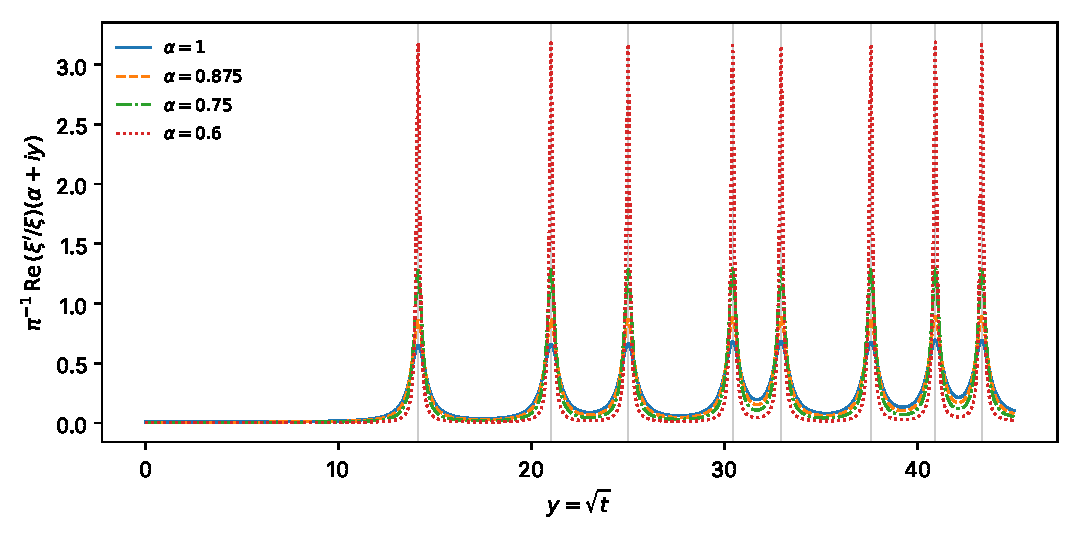
\includegraphics[width=\textwidth]{fig/nc_iw_zeta_levels.pdf}
\caption{Density $\varrho_\alpha$ for $\zeta$ at $\alpha=1,\,\frac78,\,\frac34,\,0.6$ (computed); grey lines mark the ordinates. Each bump is a Cauchy density of width $\alpha-\frac12$ that sharpens to a unit atom of $U_{1/2}$. The Thorin reading below level one is conditional on $\mathrm{QRH}(\alpha)$.}
\label{iw:fig:zeta}
\end{figure}

\begin{figure}[htbp]
\centering
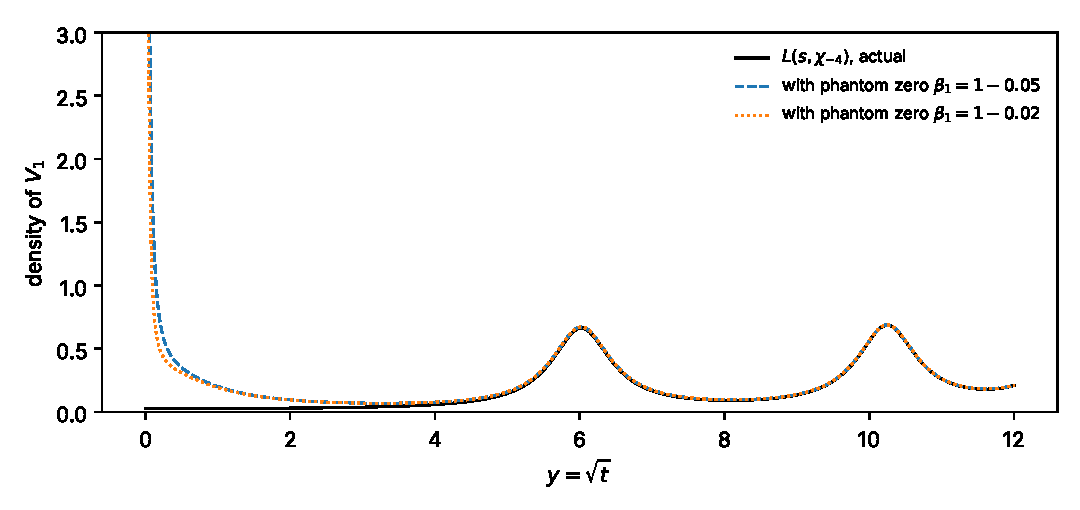
\includegraphics[width=\textwidth]{fig/nc_iw_siegel_phantom.pdf}
\caption{Density $\varrho_1$ for $L(s,\chi_{-4})$ (solid), and with a phantom real zero $\beta_1=1-\eta$ added for $\eta=0.05,\,0.02$: a near atom of mass $\frac12$ at the origin (computed).}
\label{iw:fig:siegel}
\end{figure}

\begin{figure}[htbp]
\centering
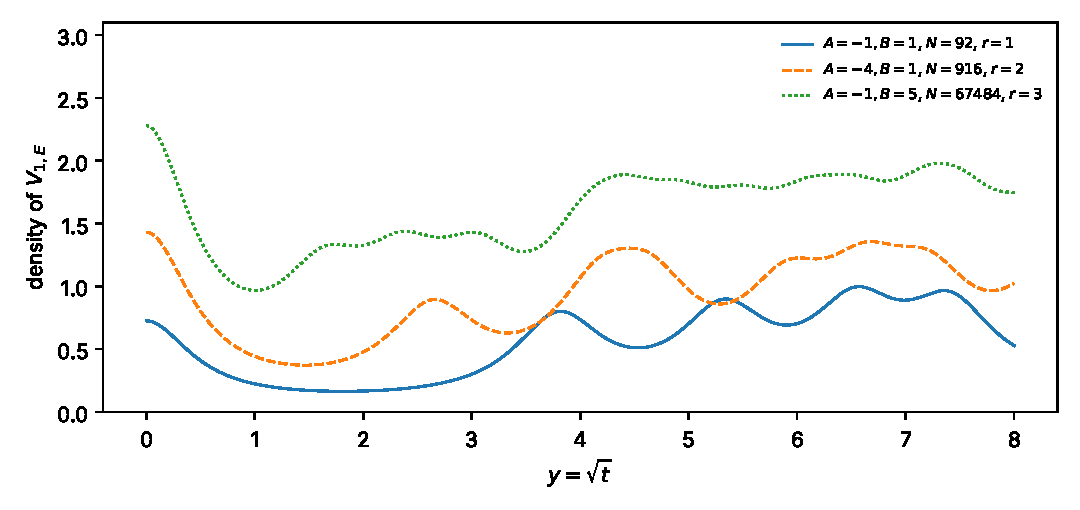
\includegraphics[width=\textwidth]{fig/nc_iw_elliptic_levels.pdf}
\caption{Density $\varrho_{1,E}$ for three curves $y^2=x^3+Ax+B^2$ of analytic rank $1,2,3$ (computed). The origin value is $\kappa_1/\pi\ge2r/\pi$.}
\label{iw:fig:elliptic}
\end{figure}

\begin{table}[htbp]
\centering\small
\begin{tabular}{rrrrrr}
\toprule
$A$ & $B$ & $N$ & $r$ & $\kappa_1$ & $\kappa_1-2r$\\
\midrule
$-1$ & 1 & 92 & 1 & 2.276 & 0.276\\
1 & 1 & 496 & 1 & 2.538 & 0.538\\
$-4$ & 1 & 916 & 2 & 4.495 & 0.495\\
6 & 4 & 6912 & 2 & 4.836 & 0.836\\
$-1$ & 5 & 67484 & 3 & 7.159 & 1.159\\
\bottomrule
\end{tabular}
\caption{Five curves of Iwaniec's family at level one (computed; the analytic ranks are numerical). The bound $\kappa_1\ge2r$ of Proposition~\ref{iw:prop:rank} holds with a small remainder from the noncentral zeros.}
\label{iw:tab:family}
\end{table}

\begin{table}[htbp]
\centering\small
\begin{tabular}{lcccccc}
\toprule
curve & $\delta=0.5$ & $0.25$ & $0.1$ & $0.05$ & $0.02$ & $0.01$\\
\midrule
$A=-1,B=1$, $r=1$ & 1.1381 & 1.0347 & 1.0056 & 1.0014 & 1.0002 & 1.0001\\
$A=-4,B=1$, $r=2$ & 2.2476 & 2.0626 & 2.0100 & 2.0025 & 2.0004 & 2.0001\\
$A=-1,B=5$, $r=3$ & 3.5794 & 3.1490 & 3.0240 & 3.0060 & 3.0010 & 3.0002\\
\bottomrule
\end{tabular}
\caption{The descent $\delta\,\kappa_{1/2+\delta}\to r$ of Proposition~\ref{iw:prop:rank} (computed), with remainder close to $\delta^2\sum_{\gamma\ne0}\gamma^{-2}$.}
\label{iw:tab:ranklimit}
\end{table}

\begin{table}[htbp]
\centering\small
\begin{tabular}{ccccc}
\toprule
$\alpha$ & $W_\alpha(\phi)$ from primes & zero side \eqref{iw:eq:Wzero} & naive Cauchy sum & $\varrho_\alpha(\gamma_1)$\\
\midrule
1.5 & 0.636 & 0.636 & 0.636 & 0.340\\
1 & 1.114 & 1.113 & 1.113 & 0.647\\
0.75 & 1.844 & 1.843 & 1.843 & 1.279\\
0.6 & 2.920 & 2.921 & 2.921 & 3.185\\
0.52 & 4.020 & 4.022 & 4.022 & 15.92\\
0.5 & 4.397 & 4.400 & 4.400 & (atom)\\
0.48 & 4.831 & 4.834 & $-4.022$ & $-15.92$\\
0.4 & 7.364 & 7.368 & $-2.921$ & $-3.185$\\
0.3 & 13.90 & 13.91 & $-2.113$ & $-1.596$\\
\bottomrule
\end{tabular}
\caption{The level $\alpha$ explicit formula for $\xi$ with the Fej\'er test function centred at $\pm\gamma_1$ (computed, one test function). The prime side \eqref{iw:eq:Wprime} agrees with the zero side at every level. Below $\frac12$ the density at $\gamma_1$ and the naive Cauchy sum are negative, but this prime side value is positive: the residue identity of Corollary~\ref{iw:cor:residue}.}
\label{iw:tab:weil}
\end{table}

\section{Is there a path to RH?}\label{iw:sec:path}

No. We say why in three parts.

The ladder. $\mathrm{QRH}(\alpha)$ is a monotone family of statements, each the Thorin measure at one level, linked by the Cauchy semigroup. A path to RH in this language is a descent of the level from $1$ (unconditional) through $\frac78$ (conditional on the unrefereed claim) and whatever Iwaniec's constructions would give, to $\frac12$. Every rung is a zero free half plane. This is the ladder analytic number theory has always climbed; the dictionary renames the rungs and adds none. Positivity at a level is equivalent to the absence of zeros to the right of it (Theorem~\ref{cx:thm:positivity}), so no property of the measures that is known short of that absence implies it (Section~\ref{qrh:sec:descent}).

What a rung costs. By Theorem~\ref{iw:thm:dictionary} $\varphi_\alpha$ is a GGC transform if and only if $\varphi_\alpha$ continues without poles to the slit plane. A fixed nonnegative test function cannot separate a zero just to the right of the level from a zero on it (Corollary~\ref{iw:cor:residue} and the estimate after it). That does not show that every test function fails: Weil's criterion is a functional built from the primes and tested on nonnegative band limited functions, and by Proposition~\ref{iw:prop:weilavg} it certifies RH at $\alpha=\frac12$. It is equivalent to RH, so using it assumes what is to be proved. Proposition~\ref{iw:prop:converse} shows that positivity at a level, even on the single family $\phi_0(y)(1\pm\cos ay)$ with $a\ge5$, is equivalent to the rung itself: the family measures the growth of $W_\alpha(\phi_0\cos a\,\cdot)$ as $a\to\infty$, and that growth is set by the rightmost zero. Proving positivity for every $a$ is therefore exactly as hard as the rung, so positivity cannot be used to climb. The computational checks of Volume~II that compare the deconvolved measure with the zero measure in total variation test finitely many functions with transforms in a bounded range; they are consistent with $\mathrm{QRH}(\alpha)$ and cannot prove it.

Where leverage could come from. A Thorin path would have to supply a property $\mathcal P$ of the measures $D_\alpha$ that holds for every $\alpha>1$ and persists under a small step down in level. When $\alpha$ exceeds the real part of every zero, the deconvolution form of RH (Theorem~\ref{tf:thm:deconv}(a), stated there for $\xi$) says that a nonnegative $\nu$ with $D_\alpha=P_\varepsilon*\nu$ exists if and only if $\mathrm{QRH}(\alpha-\varepsilon)$, and then $\nu=D_{\alpha-\varepsilon}$. A hypothesis that merely asks the signed solution of $D_\alpha=P_\varepsilon*\nu$ to be nonnegative is vacuous when no solution exists, so the content of any property $\mathcal P$ must include the existence of the nonnegative deconvolution, which is the conclusion. Positivity of the density alone fails for this reason, and log concavity in $y$ fails for $\alpha$ near $\frac12$ because the density has a bump at each ordinate, and at larger levels for a different reason, the almost periodic second derivative of the prime sum. Hyperbolic complete monotonicity of $\varphi_\alpha$ cannot serve as $\mathcal P$: by Theorem~\ref{iw:thm:dictionary} and Bondesson's characterisation \cite[Theorem 6.1.1]{Bondesson} it is equivalent to $\mathrm{QRH}(\alpha)$ at every level $\alpha\ge\frac12$ (this extends Corollary~\ref{cor:hcm} and Theorem~\ref{bh:thm:main}), so it is the conclusion (proved). Its real axis consequence, complete monotonicity of $-\varphi_\alpha'/\varphi_\alpha$, is infinite divisibility of the level $\alpha$ law (proved), and at $\alpha=\frac12$ it does not imply the Riemann hypothesis: Theorem~\ref{thm:ch13:perturb} gives an even entire function with the order, type and reflection symmetry of $\xi$, with zeros off the critical line, whose reciprocal clock is nevertheless infinitely divisible. One step of the descent needs a hypothesis stated. Assume $\mathrm{QRH}(\alpha)$ and that no zero lies on $\re s=\alpha$. Then $\mathrm{QRH}(\alpha-\varepsilon)$ holds, with zeros on $\re s=\alpha-\varepsilon$ allowed, if and only if $\varrho_\alpha$ continues analytically without poles to $|\Im y|<\varepsilon$, and then $\varrho_{\alpha-\varepsilon}(y)=2\,\re\varrho_\alpha(y+i\varepsilon)-(P_\varepsilon*\varrho_\alpha)(y)$ (Theorems~\ref{cd:thm:herglotz} and \ref{tf:thm:deconv}, with $\varrho_{\alpha+\varepsilon}=P_\varepsilon*\varrho_\alpha$ from Theorem~\ref{iw:thm:semigroup}; proved). If a zero lies on $\re s=\alpha$ then $D_\alpha$ has an atom and neither the analyticity nor the continuation holds. Nothing here proves that any other property persists under a step down (heuristic). Section~\ref{rg:sec:level} makes this precise for the family of Proposition~\ref{iw:prop:converse}: the step is one inequality on level $\alpha$ data, and positivity at level $\alpha$ (at $\alpha=1$ unconditionally) together with the functional equation and a positive prime measure does not give it.

\begin{remark}[caps uniform in height are impossible]\label{iw:rem:nocap}
Let $\frac12<\alpha\le1$, assume $\mathrm{QRH}(\alpha)$ for $\xi$ and that no zero lies on $\re s=\alpha$ (otherwise $D_\alpha$ has atoms and no density bound holds for it). Then $\sup_y\big[\varrho_\alpha(y)-\frac1{2\pi}\log\frac{|y|+2}{2\pi}\big]=+\infty$, so no bound of the form mean density plus a constant holds for all real $y$ at any such level. Status: proved. This is the chapter's observation, following an unrefereed note of Polson (November 2026), whose argument used the density of the values of $\zeta$ on a vertical line \cite{BohrCourant}; the route below needs only Kronecker's theorem. Suppose $\varrho_\alpha(y)\le\frac1{2\pi}\log\frac{|y|+2}{2\pi}+K$ for all $y$. By Theorem~\ref{iw:thm:semigroup}, for $1<u\le2$ we have $\varrho_u=P_{u-\alpha}*\varrho_\alpha$, and smoothing at width at most $2$ changes a function of logarithmic growth by a bounded amount, so the same bound holds with $K+C_1$. Write $\xi=G\zeta$. By Stirling and since the term $1/(s-1)$ of $G'/G$ has bounded real part for $|y|\ge1$, $\re G'/G(u+iy)\ge\frac12\log\frac{|y|+2}{2\pi}-C_2$ for $|y|\ge1$, hence $\re\zeta'/\zeta(u+iy)=\pi\varrho_u(y)-\re G'/G(u+iy)\le C_3$ for all $1<u\le2$ and $|y|\ge1$. On the other hand $-\re\zeta'/\zeta(u+iy)=\sum_p\log p\,p^{-u}\cos(y\log p)+O(1)$ uniformly in $u>1$, and the numbers $\log p$ are linearly independent over $\mathbb Q$, so by Kronecker's theorem for every $P$ and $\delta>0$ there are arbitrarily large $y$ with $y\log p$ within $\delta$ of $\pi$ modulo $2\pi$ for all $p\le P$. Letting $\delta\to0$ and then $P\to\infty$ gives $\sup_{|y|\ge1}\re\zeta'/\zeta(u+iy)\ge\sum_p\log p\,p^{-u}-C\ge\frac1{u-1}-C'$, which contradicts $\re\zeta'/\zeta\le C_3$ as $u\downarrow1$. Consequently a pointwise lower bound $\varrho_\alpha(\gamma)\ge1/(\pi(\alpha-\beta))$ at a hypothetical zero, combined with an upper bound uniform in $y$, gives only regions that shrink with height, as in Proposition~\ref{tx3:prop:dvp} and Theorem~\ref{cf:thm:dvp} (de la Vall\'ee Poussin in Thorin form). Caps bounded only at zero ordinates, or outside an exceptional set of $y$, are not ruled out.
\end{remark}

\section{Open problems}\label{iw:sec:open}

\begin{problem}[family deconvolution test]\label{iw:prob:family}
For $A\approx X^{1/3}$, $B\approx X^{1/4}$ on the double zero progressions, compute the family average $\overline D_\alpha$ at a level $\alpha>1$ from averages of $a_E(p)$ (the Dirichlet series of $\Lambda_E'/\Lambda_E$ is not absolutely convergent at $\alpha=1$) and invert the semigroup of Theorem~\ref{iw:thm:semigroup} down to level $\frac12$. The recovered measure has an atom at the origin of mass $\overline r\ge2$ on the progressions, under GRH for the family. An analogue of Theorem~\ref{iw:thm:weil} for $\Lambda_E$, not proved here, would say that the prime side functional at level $\frac12$ reproduces $\int\phi\,d\overline D_{1/2}$ for band limited $\phi$ and that the atom appears as $\phi(0)\overline r$. The open question is the rate at which the recovered atom converges to $\overline r$ as the support $X$ grows.
\end{problem}
